\documentclass[journal]{IEEEtran}
\usepackage[cm]{fullpage}
\usepackage[utf8]{inputenc}
\usepackage[english]{babel}
\usepackage{url}
\usepackage{graphicx}
\graphicspath{ {../images/} }

\usepackage[noadjust]{cite}

\usepackage{multicol}
\usepackage{hyperref}
\hypersetup{
    %backref,
    pdfstartview=FitH,
    pdfpagemode=UseNone,
    %colorlinks=true,
    %bookmarks=true,
    pdftitle={Project proposal --- Fabricator of an pure electric hybrid vehicle},
    pdfauthor={Suresh Kumar Gadi},
    pdfsubject={electric vehicle},
    pdfkeywords={electric vehicle, energy management, super capacitors, power electronics},
    pdfstartpage = 2
}

\usepackage{tcolorbox}



\title{Project proposal --- Fabricator of an pure electric hybrid vehicle}
\date {January 10, 2017}
\author{Dr. Suresh Kumar Gadi}
\begin{document}
\maketitle
\begin {abstract}
This document identifies the requirements for fabricating an electric car at FIME, UAdeC. Also, proposes a possible methodology to realize the project.
\end {abstract}
\section{Objective}
The objective of this project is to model, design and fabricate an pure electric hybrid vehicle with the following functionality.
\begin{itemize}
	\item Steep acceleration curves similar to the petroleum vehicles (PV).
	\item Maximizing the energy harvesting at all the times, i.e. during all kinds of the breaking routine.
\end{itemize}
\section{Introduction}
The electric vehicles were introduced in the early nineteenth century; these were holding a greater market in comparison to the internal combustion (IC) ones until the end of that century \cite{6487583}. However, petroleum vehicles (PV) soon became more common on the roads later, which can be seen from the 2005 estimates, which indicate that the PV constitute a 97\% of the vehicles \cite{de2012electrical}. Recently there is a growing interest in the hybrid vehicles (a hybrid of petroleum and electric) and pure electric vehicles (PEV) \cite{hori2004future, turrentine1995will, SKGadi-2016EuropeReportEV}.
\section{Selection of storage type}
\begin{figure}[h]
	\centering
	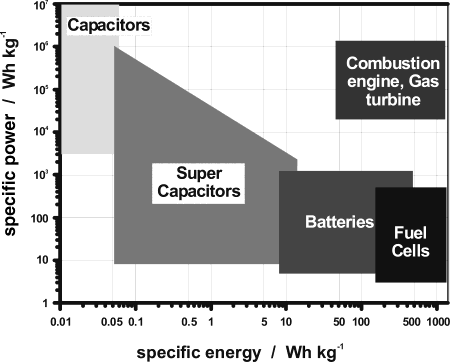
\includegraphics[width=0.48\textwidth]{specific-power-energy}
	\caption{Ragone plot --- Comparison energy density (specific energy) and power density (specific power) of most common storage domains \cite{winter2004batteries}.}
	\label{Fig:power-vs-energy-1}
\end{figure}

\begin{figure}
	\centering
	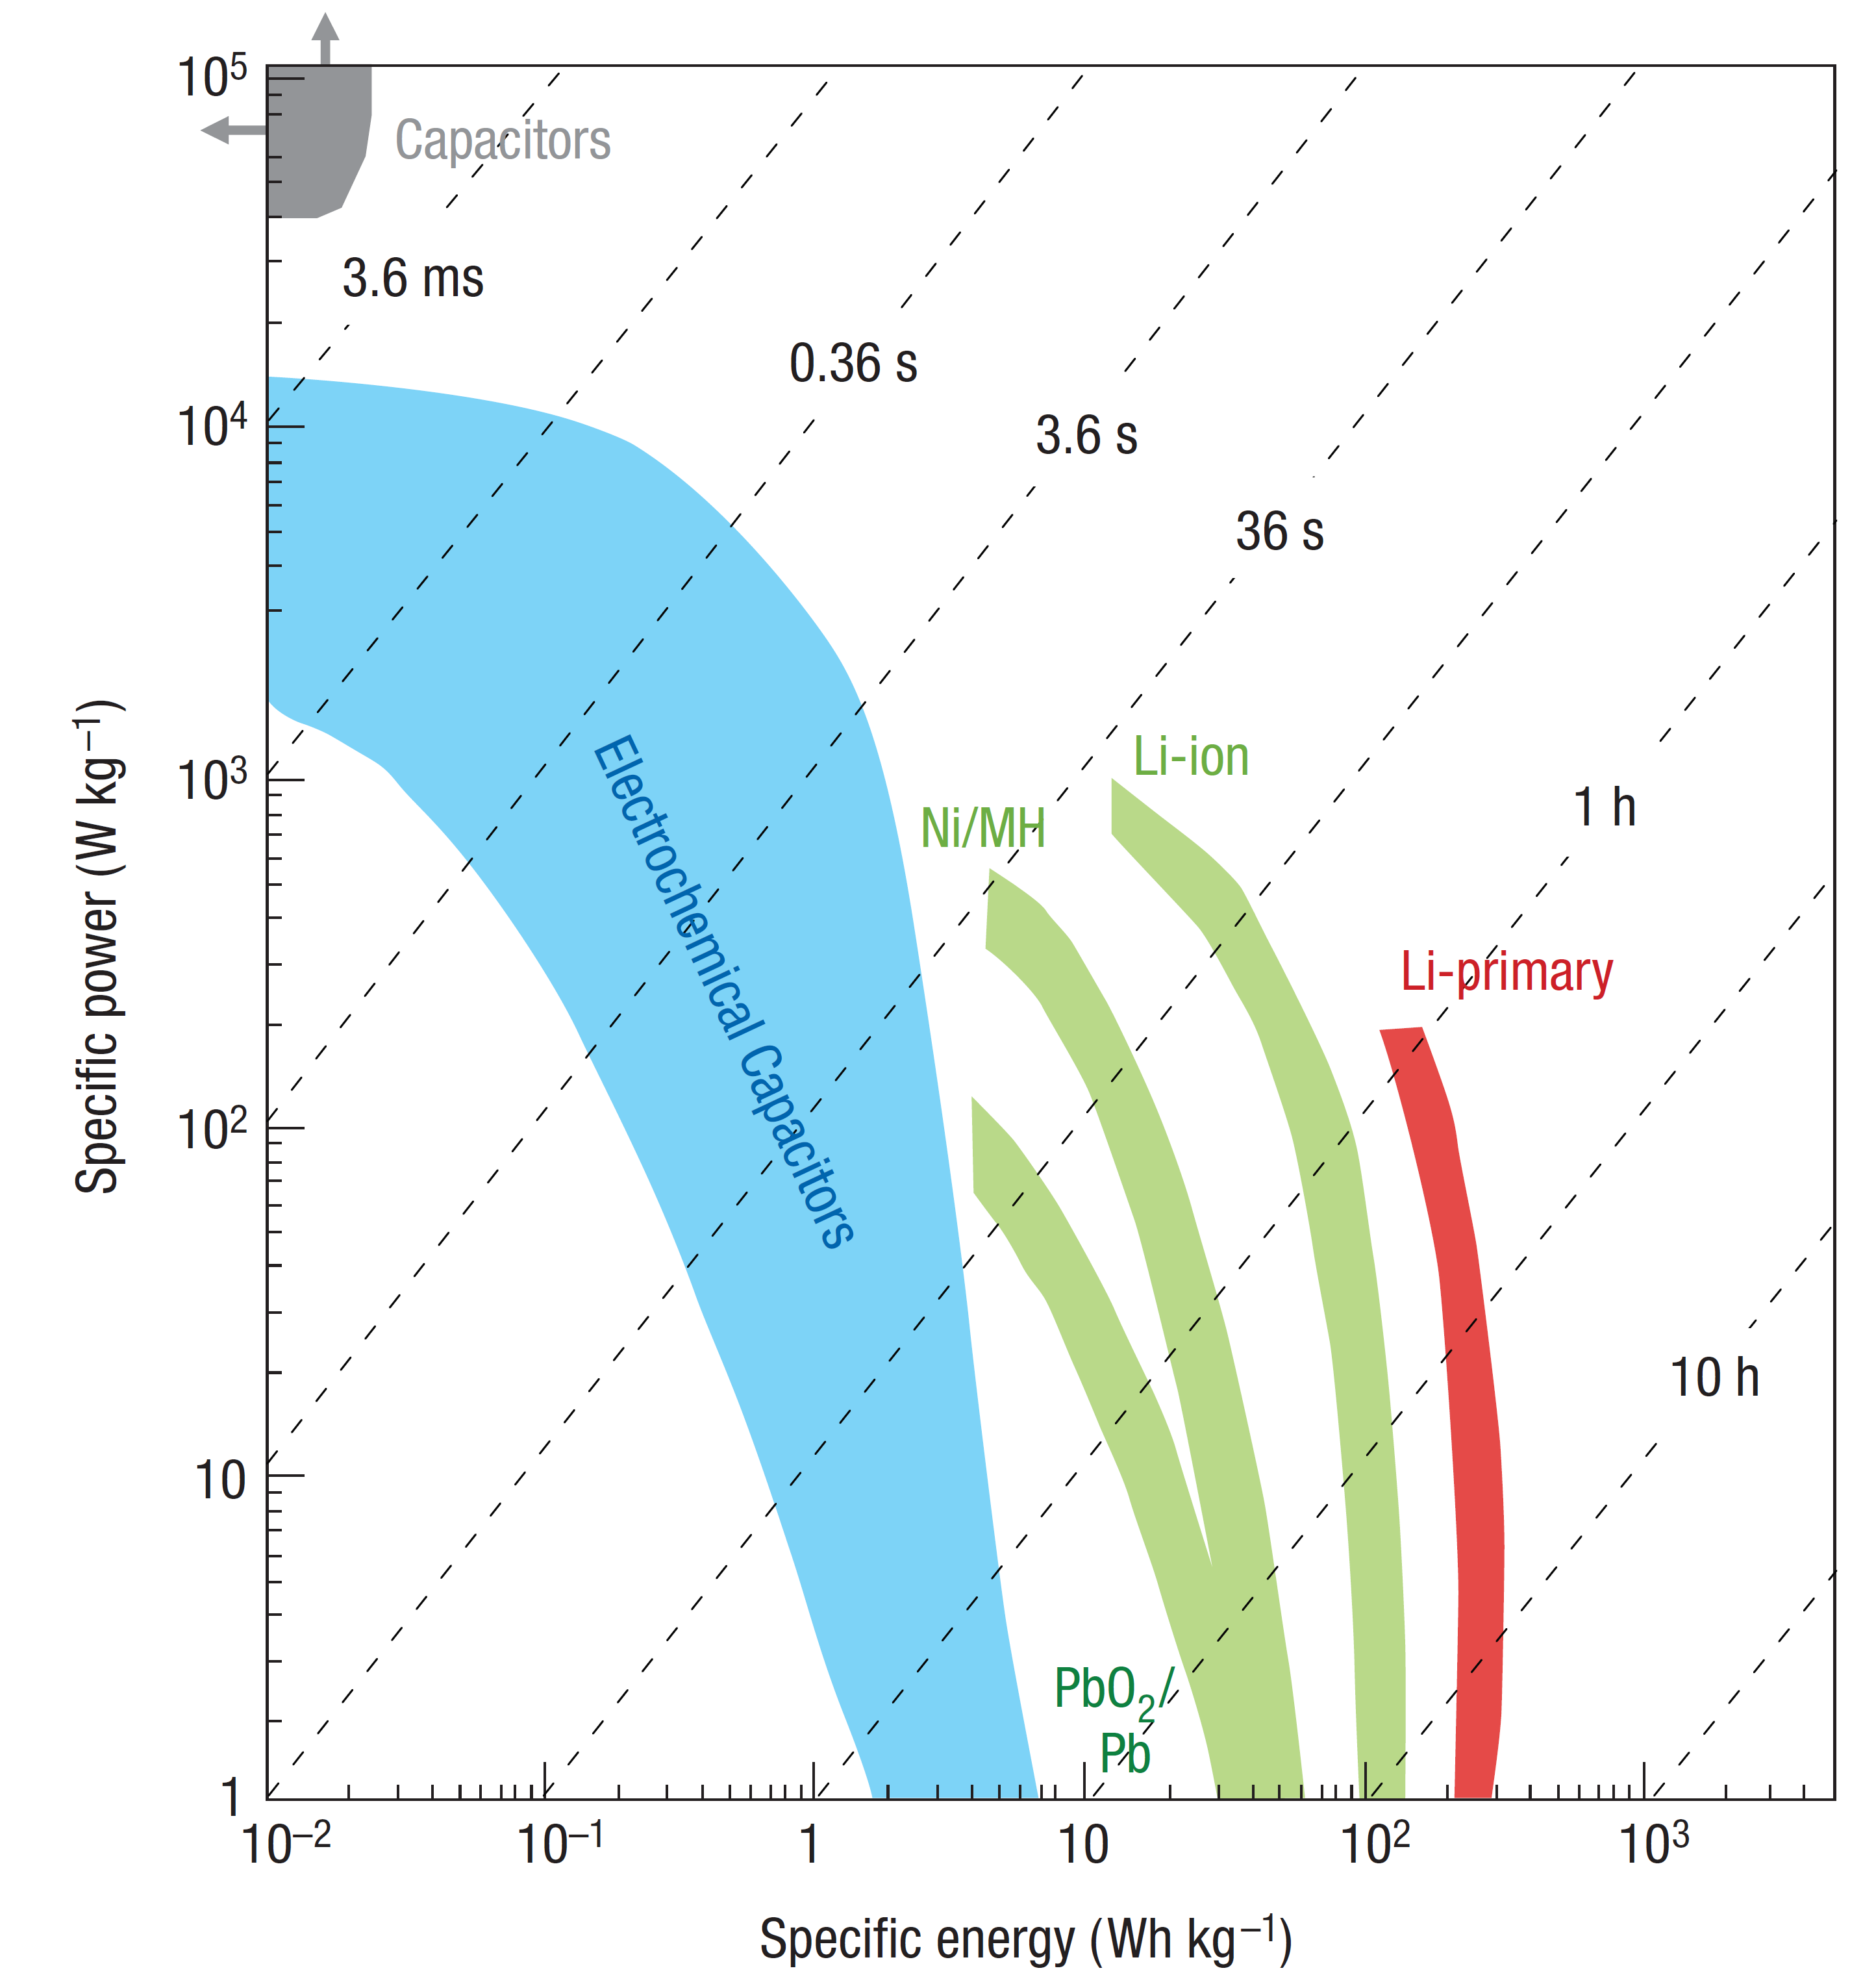
\includegraphics[width=0.48\textwidth]{power-vs-energy-density}
	\caption{Ragone plot --- Comparison energy density (specific energy) and power density (specific power) of various electric power storages \cite{simon2008materials}.}
	\label{Fig:power-vs-energy-2}
\end{figure}
\autoref{Fig:power-vs-energy-1} shows the Ragone plot for the most common storage domains \cite{simon2008materials}. It is clear that combustion engines have high specific power and specific energy. In the context of automobiles, specific energy can be associated to the fuel autonomy measure, i.e. the distance it can move by consuming a unit fuel mass, and the specific power can be associated to the acceleration which it can achieve with a given unit fuel mass. So from \autoref{Fig:power-vs-energy-1}, we see that a petroleum based automobile have an advantage over any other domain. Also, we can see that a properly designed electric hybrid system can perform on par with combustion engines.

\autoref{Fig:power-vs-energy-2} shows the Ragone plot of electric storage devices. We can ignore the Li-primary batteries option because they are not rechargeable. So, the solution to achieve high specific energy and specific power is combining the positive trades of the super-capacitors (electrochemical capacitors) and the Li-ion batteries in an hybrid system.
\section{Power flow in an EV}
\begin{figure}
	\centering
	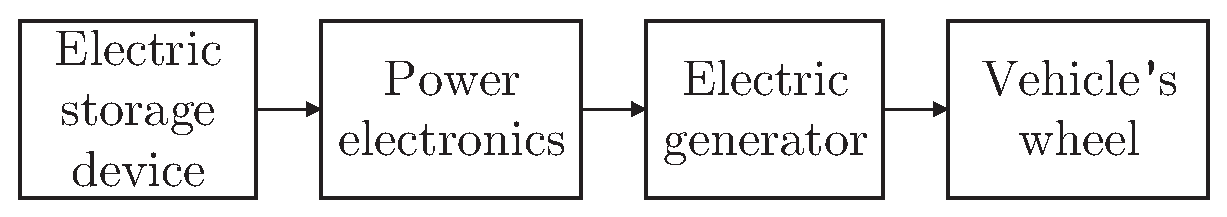
\includegraphics[width=0.48\textwidth]{driving-mode-scheme}
	\caption{Power flow diagram of an EV in the driving mode}
	\label{Fig:driving-mode-scheme}
\end{figure}
\begin{figure}
	\centering
	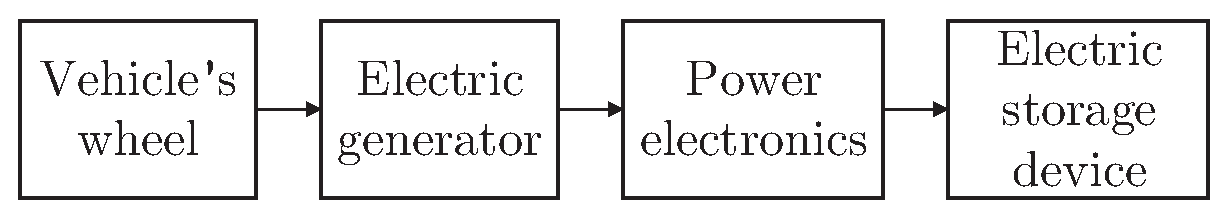
\includegraphics[width=0.48\textwidth]{braking-mode-scheme}
	\caption{Power flow diagram of an EV in the braking mode}
	\label{Fig:braking-mode-scheme}
\end{figure}
\begin{figure}
	\centering
	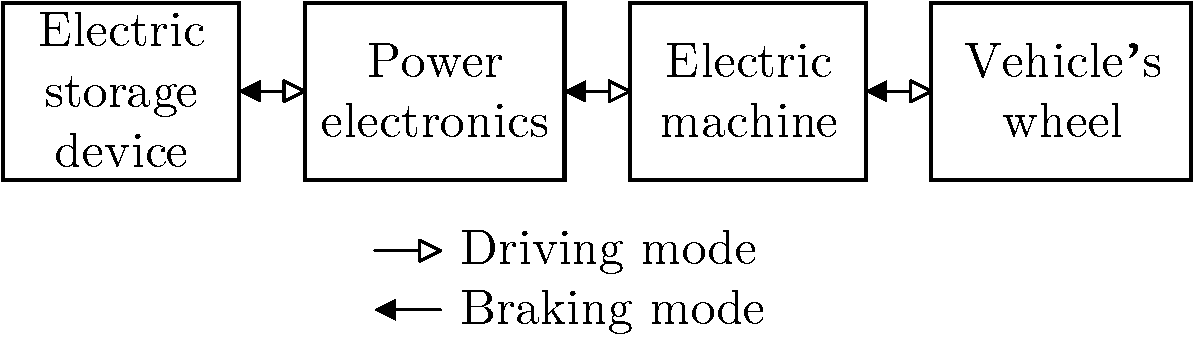
\includegraphics[width=0.48\textwidth]{combining-driving-n-braking-modes}
	\caption{Schematic showing the EV's power flow diagram}
	\label{Fig:combining-driving-n-braking-modes}
\end{figure}
At any given time a vehicle operates in one of the two modes, namely the driving mode and the braking mode. In an EV the wheel is coupled to the electric machine. Hence, in the driving mode the electric machine should act as a motor and in the driving mode it should act as a generator. \autoref{Fig:driving-mode-scheme} and \autoref{Fig:braking-mode-scheme} show the power flow diagram for an electric vehicle in the driving mode and the braking mode respectively.

\autoref{Fig:combining-driving-n-braking-modes} shows a possible way of merging both modes of operations in a vehicle. In order to achieve this scheme, we need to satisfy the following conditions.

\begin{tcolorbox}[colback=blue!0!white,colframe=blue!75!black,title=Conditions]
\begin{enumerate}
  \item The coupling between electric machine and the vehicle's wheel should be bidirectional.
  \item The same electric machine should work as a motor and a generator.
  \item The power electronics should be bidirectional.
\end{enumerate}
\end{tcolorbox}

\section{Selection of the electric machine}
The electric machines capable of acting as both motors and generators are:
\begin{itemize}
  \item AC induction motor
  \item AC synchronous machine
  \item DC machines
\end{itemize}
\subsection{AC induction motor}
An induction motor required a speed higher than the synchronous speed to act as a generator, hence this is not viable in our design.
\subsection{AC synchronous machine}
AC synchronous machine require the following power electronic modules.
\begin{itemize}
  \item Rectifiers (AC to DC converters)
  \item Inverters (DC to AC converters)
  \item DC to DC converter (Buck–boost converter)
\end{itemize}
\subsection{DC machines}
DC machines require the following power electronic modules.
\begin{itemize}
  \item DC to DC converter (Buck–boost converter)
\end{itemize}

We select DC machine to minimize the system complexity.

\section{System design}

\begin{figure}
	\centering
	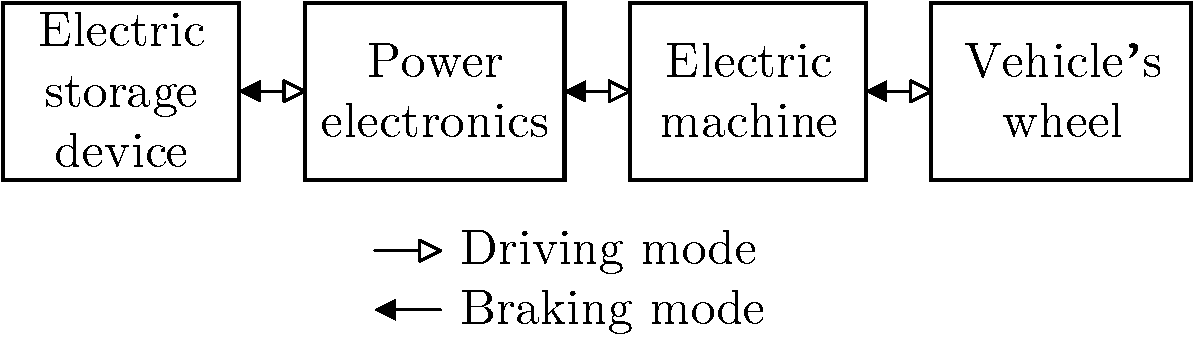
\includegraphics[width=0.48\textwidth]{combining-driving-n-braking-modes}
	\caption{Schematic showing the EV's power flow diagram}
	\label{Fig:combining-driving-n-braking-modes}
\end{figure}
Figure x shows the complete system scheme. Here for simplicity, one one direction of wheel movement is considered. We can notice that we need the following for the EV.
\begin{tcolorbox}[colback=blue!0!white,colframe=blue!75!black,title=Conditions]
\begin{enumerate}
  \item The coupling between electric machine and the vehicle's wheel should be bidirectional.
  \item The same electric machine should work as a motor and a generator.
  \item The power electronics should be bidirectional.
\end{enumerate}
\end{tcolorbox}

\section{s}

\bibliographystyle{IEEEtran}
\bibliography{../refs}

\end{document} 